\section{Heuristiques en ligne}
Afin de permettre un calcul rapide, les heuristiques sont un compromis entre rapidité et fiabilité. En effet, une heuristique est une méthode de calcul rapide, sans toutefois être exact ou optimal. L'association Tournesol souhaite ici mettre en place une heuristique permettant, dès qu'une comparaison est opérée, le calcul et la mise à jour des scores concernés.

\subsection{Première heuristique}

Les conditions du premier ordre de la maximisation de la vraisemblance \textit{a posteriori} (\ref{equation:cpo}) donnent en regroupant les termes en $\theta^{*}_a$ à gauche :

\begin{equation}
 \forall a \in A,   (\alpha_{prior} + \sum_{ab \in AB} k_{ab}) \theta^{*}_a = \sum_{ab \in AB} k_{ab}(\theta^{*}_b + \ell(\Tilde{r_{ab}}))
\end{equation}

Au lieu de résoudre simultanément le système d'équations, où l'inversion matricielle est de l'ordre de $\mathcal{O}(n^3)$\footnote{Les meilleurs algorithmes sont de l'ordre de $\mathcal{O}(n^{2.373})$}, l'idée est d'appliquer une descente de coordonnées à partir du dernier état connu, idéalement à partir des coordonnées exactes données par l'algorithme Mehestan. 

Comme l'heuristique consiste à mettre à jour le score de a et b pour une comparaison entre ces deux dernières entités, les scores de a et b sont mis à jour à partir des scores précédents des entités connexes, en itérant $\tau$ fois en cercle concentrique dans le graphe de connexité.

\begin{equation}
  \forall e \in \set{a,b}, \theta^{heuristique}_e = \sum_{ab \in AB} k_{ab}(\theta^{dernier score}_b + \ell(\Tilde{r_{ab}})) (\alpha_{prior} + \sum_{ab \in AB} k_{ab})^{-1}
\end{equation}

\pagebreak

\begin{algorithm}
\renewcommand{\algorithmcfname}{Algorithme}
\caption{Heuristique pour le calcul des scores individuels de a et de b et des incertitudes par descente de coordonnées}\label{alg:local_scores_matrix_inversion}
\KwData{la matrice de comparaison $r_t$, l'hyperparamètre de l'a priori $\alpha_{prior}$, les scores précédents $\score$, $\tau$ le nombre d'itérations}
\KwRes{les scores individuels de a et b $\scoreh$ et leur incertitude $\deltascoreh$}

$ Ensemble \leftarrow \set{a,b}$

$ Iteration \leftarrow 1$

$ \scoreh_0 \leftarrow \score $

\Tq{$Iteration \leq \tau$}{


$ \scoreh_{Iteration} \leftarrow \scoreh_{Iteration-1} $

\PourCh{$element \in Ensemble$}{

$\Tilde{r_t} \leftarrow r_t/(1+R_{max})$

$\ell_t \leftarrow -\Tilde{r_t}/\sqrt{1-\Tilde{r_t}^2}$

$k_t \leftarrow (1-\Tilde{r_t}^2)^3$

$K_{aa,t} \leftarrow \alpha_{prior} + \sum_{b \in N(A)} k_{ab,t}$

$L_t \leftarrow \sum_{b \in N(A)} k_{ab,t}l_{ab,t}$


$\scoreh_{element,Iteration} \leftarrow  (L_t + \sum_{b \in N(A)}k_{ab,t}\scoreh_{Iteration-1})/K_{aa,t}$

$\deltascoreh_{element,Iteration} \leftarrow \frac{1}{card(AB)} \left( 1 + \sum_{ab \in AB} k_{ab,t}(l_{ab,t} - \scoreh_{ab,Iteration-1})^2 \right)$

}

$Ensemble \leftarrow Voisinage(Ensemble) \cup Ensemble $

$Iteration \leftarrow Iteration + 1$

}


$ \scoreh \leftarrow \scoreh_\tau $

$ \deltascoreh \leftarrow \deltascoreh_\tau $


\Return{$\scoreh,\deltascoreh$}
\end{algorithm}

\subsection{Proposition d'estimateurs mesurant la qualité de l'heuristique}


\subsubsection{Biais de somme nulle}

Les comparaisons relatives constituent un système à somme nulle, puisque des quantités sont ajoutées et retirées de manière asymétrique. Les scores individuels bruts sont à somme nulle. En cas de somme non nulle, le biais signifie que des scores sont sous-estimés ou sur-estimés sans justification valable. Par conséquent, par exemple, si les scores d'une entité sont sous-estimés par plusieurs contributeurs, alors le score global de l'entité peut être lui aussi sous-estimé. Il convient alors de mesurer et de maîtriser cette déformation des poids dans un premier temps d'une manière grossière.

Soit l'indicateur \gls{bsn},

\begin{equation}
BSN= \sum_{a \in A} \theta^{heuristique}_{a}
\end{equation}


\subsubsection{Somme des écarts absolus entre résultats de l'heuristique et de Mehestan}

Comme l'heuristique permet d'avoir des résultats approchés des scores calculés Mehestan, la somme des écarts absolus constitue une mesure de la convergence entre les deux algorithmes. Idéalement, cet indicateur devrait tendre vers zéro si possible. Dans le cas contraire, il est nécessaire de mesurer à quel point les résultats de l'heuristique s'écartent des scores réels et d'affiner l'heuristique pour diminuer l'écart.

Soit l'indicateur \gls{eam},
\begin{equation}
EAM= \sum_{a \in A} \left| \theta^{heuristique}_{a}-\theta^{Mehestan}_{a} \right| 
\end{equation}



De plus, la somme des écarts absolus des incertitudes donne une idée de la déformation de l'intervalle de confiance.


En outre, la somme des écarts sous-estimés et la somme des écarts sur-estimé constituent des mesures complémentaires riches en information.

\subsubsection{Temps de rapidité de l'heuristique}

Une heuristique doit être suffisamment rapide pour la plateforme Tournesol pour permettre d'être joué plusieurs fois par contributeur et en concurrence avec d'autres contributeurs.


\subsection{Calcul théorique de l'heuristique proposée}
%\subsubsection{Evaluation des bornes sur l'estimateur \gls{BSN}}

\subsubsection{Ajout d'un premier score}

Soit un contributeur \textit{i} ayant fait une comparaison entre $E_{1}$ et $E_{2}$ avec une notation $n_{1-2} \in [\![-10;10]\!]$

$r_{t+1}= \begin{pmatrix}
0 & n_{1-2} \\
-n_{1-2} & 0 
\end{pmatrix}$

$l_{t+1}= \begin{pmatrix}
0 & l_1 \\
-l_1 & 0 \\
\end{pmatrix}
$

$k_{t+1}= \begin{pmatrix}
0 & k_1 \\
k_1 & 0 \\
\end{pmatrix}
$


$L_{t+1}= \begin{pmatrix}
l_1 k_1\\
-l_1 k_1 \\
\end{pmatrix} \triangleq
\begin{pmatrix}
L1\\
L2
\end{pmatrix} 
$

$K_{aa,t+1}= \begin{pmatrix}
\alpha + k_1\\
\alpha +  k_1\\
\end{pmatrix} \triangleq
\begin{pmatrix}
K1\\
K2
\end{pmatrix} 
$

avec les scores bruts individuels calculés par l'algorithme Mehestan (cf Exemple \ref{example:n1})

$\score_{t+1}= \begin{pmatrix}
\score_{t+1,1} \\
\score_{t+1,2} 
\end{pmatrix}=
\begin{pmatrix}
l_1k_1 / (\alpha + 2k_1)\\
-l_1k_1 / (\alpha + 2k_1)\\
\end{pmatrix}$

L'heuristique donne pour $\tau=0, A^{t+1,0}=\set{E_1,E_2}$

\begin{equation*}
\scoreh_{t+1,0}= \begin{pmatrix}
(L_1+\score_{1} k_1) / K_1 \\
(L_2+\score_{2} k_1) / K_2
\end{pmatrix}
\end{equation*}

pour $\tau=1, A^{t+1,1}=\set{E_1,E_2}$


\begin{equation*}
\scoreh_{t+1,1}= \begin{pmatrix}
(L_1+\scoreh_{t+1,0,1} k_1) / K_1 \\
(L_2+\scoreh_{t+1,0,2} k_1) / K_2
\end{pmatrix}
\end{equation*}

\begin{equation*}
\gls{bsn}=0
\end{equation*}


car  $(L_1+\score_{1} k_1) / K_1 = -(L_2+\score_{2} k_1) / K_2$

puis 
$(L_1+\scoreh_{t+1,0,1} k_1) / K_1 = -(L_2+\scoreh_{t+1,0,2} k_1) / K_2 $

$\gls{eam}=  |\score_{t+1,1} - \scoreh_{t+1,1,1}|   +  |\score_{t+1,2} - \scoreh_{t+1,1,2}| $
\begin{equation*}
\forall{n_{1-2}}\in [\![-10;10]\!], EAM \in [0,0.842]
\end{equation*}

Le minimum et le maximum sont atteints respectivement en $n_{1-2}=0$ et en -8 ou 8.

%%%%%%%%%%%%%%%%%%%%%%%%%%%% Cas 3dim %%%%%%%%%%%%%%%%%%%%%%%%%%%%%%%%%%

\subsubsection{Ajout d'un score après calcul par Mehestan}


Soit un contributeur \textit{i} ayant fait une comparaison entre $E_{1}$ et $E_{2}$ avec une notation $n_{1-2} \in [\![-10;10]\!]$


$r_{t}= \begin{pmatrix}
0 & n_{1-2} \\
-n_{1-2} & 0 
\end{pmatrix}$

avec les scores bruts individuels calculés par l'algorithme Mehestan

$\score_{t}= \begin{pmatrix}
\score_{t,1} \\
\score_{t,2} 
\end{pmatrix}$

Le contributeur effectue une nouvelle comparaison entre $E_{2}$ et $E_{3}$ avec une notation $n_{2-3} \in [\![-10;10]\!]$. Les scores sont cette fois-ci calculés par l'heuristique.

$r_{t+1}= \begin{pmatrix}
0 & n_{1-2} & 0\\
-n_{1-2} & 0 & n_{2-3}\\
0 & -n_{2-3} & 0
\end{pmatrix}$

$l_{t+1}= \begin{pmatrix}
0 & l_1 & 0\\
-l_1 & 0 & l_2\\
0 & -l_2 & 0
\end{pmatrix}
$

$k_{t+1}= \begin{pmatrix}
0 & k_1 & 0\\
k_1 & 0 & k_2\\
0 & k_2 & 0
\end{pmatrix}
$

avec 

$l_1= -\tilde{r_1}/\sqrt{(1-\tilde{r_1}²)}$

et $k_1= (1-\tilde{r_1}²)³ $

et $\tilde{r_1} = n_{1-2}/(R_{max}+1)$

et ici $R_{max}=10$

$l_{t+1} \cdot k_{t+1}= \begin{pmatrix}
0 & l_1 k_1 & 0\\
-l_1 k_1 & 0 & l_2 k_2\\
0 & -l_2 k_2 & 0
\end{pmatrix}
$

$L_{t+1}= \begin{pmatrix}
l_1 k_1\\
-l_1 k_1 +l_2 k_2\\
-l_2 k_2
\end{pmatrix} \triangleq
\begin{pmatrix}
L1\\
L2\\
L3
\end{pmatrix} 
$

$K_{aa,t+1}= \begin{pmatrix}
\alpha + k_1\\
\alpha +  k_1 + k_2\\
\alpha + k_2
\end{pmatrix} \triangleq
\begin{pmatrix}
K1\\
K2\\
K3
\end{pmatrix} 
$



Pour $\tau=0, A^{t+1,0}=\set{E_2,E_3}$

$ \scoreh_{t+1,0}= \begin{pmatrix}
(L_2+\score_{1} k_1) / K_2 \\
(L_3+\score_{2} k_2) / K_3
\end{pmatrix}

avec $\score_{1} = - \score_{2} = l_1 k_1/(\alpha + 2 k_1)&

Pour $\tau=1, A^{t+1,1}=\set{E_1,E_2,E_3}$

$ \scoreh_{t+1,1}= \begin{pmatrix}
(L_1+\scoreh_{t+1,0,2} k_1) / K_1 \\
(L_2+\score_{1} k_1) / K_2 \\
(L_3+\scoreh_{t+1,0,2} k_2) / K_3 
\end{pmatrix}

$BSN =
(L_1+\scoreh_{t+1,0,2} k_1) / K_1 +
(L_2+\score_{1} k_1 + \scoreh_{t+1,0,2} k_2)  / K_2 +
(L_3+\scoreh_{t+1,0,2} k_2) / K_3 
$

\begin{equation*}
    \forall{n_{1-2},n_{2-3}}\in [\![-10;10]\!]² , BSN \in [-1.10,1.10]
\end{equation*}


Le minimum et le maximum sont atteints respectivement en $(n_{1-2},n_{2-3})=(-4, -9)$ et en (4, 9).


scores de Mehestan

$K_{t+1} \score_{t+1}= L_{t+1}$

$\score_{t+1}=K^{-1}_{t+1} L$

avec 
$ K_{t+1}= \begin{pmatrix}
K_1&-k_{12}&-k_{13}\\
-k_{12}&K_2&-k_{23}\\
-k_{13}&-k_{23}&K_3
\end{pmatrix}

ici, $k_{12}=k1, k_{13}=0, k_{23}=k2$
alors, 

$ K_{t+1}= \begin{pmatrix}
K_1&-k_1&0\\
-k_1&K_2&-k_2\\
0&-k_2&K_3
\end{pmatrix}

$ K^{-1}_{t+1}= \left( \begin{array}{ccc} K_1 K_2-k_2^2 & k_1 K_2 & k_1 k_2 \\ k_1 K_2 & K_2 K_3 & k_2 K_3 \\ k_1 k_2 & k_2 K_3 & K_1 K_3-k_1^2 \end{array} \right)/(-K_2 k_1^2-k_2^2 K_3+K_1 K_2 K_3)$


EAM=  $|\score_{t+1,1} - \scoreh_{t+1,1,1}|   +  |\score_{t+1,2} - \scoreh_{t+1,1,2}|  +  |\score_{t+1,3} - \scoreh_{t+1,1,3}|  $

\begin{equation*}
\forall{n_{1-2},n_{2-3}}\in [\![-10;10]\!]²  EAM \in [ 0.000,1.640 ]
\end{equation*}


Le minimum et le maximum sont atteints respectivement en $(n_{1-2},n_{2-3})=(0, 0)$ et en (-9, -7).



%%%%%%%%%%%%%%%%%%%%%%%%%%%%%%% VARIANTE %%%%%%%%%%%%%%%%%%%%%%%%%%%%%%%%





Variante : 
Le contributeur effectue une nouvelle comparaison entre $E_{1}$ et $E_{3}$ avec une notation $n_{1-3} \in [\![-10;10]\!]$. Les scores sont cette fois-ci calculés par l'heuristique.

$r_{t+1}= \begin{pmatrix}
0 & n_{1-2} &  n_{1-3} \\
-n_{1-2} & 0 & 0\\
 -n_{1-3}  & 0 & 0
\end{pmatrix}$

$l_{t+1}= \begin{pmatrix}
0 & l_1 & l_2\\
-l_1 & 0 & 0\\
-l_2 & 0 & 0
\end{pmatrix}
$

$k_{t+1}= \begin{pmatrix}
0 & k_1 &  k_2 \\
k_1 & 0 & 0 \\
 k_2 & 0 & 0
\end{pmatrix}
$


$l_{t+1} \cdot k_{t+1}= \begin{pmatrix}
0 & l_1 k_1 & l_2 k_2\\
-l_1 k_1 & 0 & 0\\
-l_2 k_2 & 0 & 0
\end{pmatrix}
$

$L_{t+1}= \begin{pmatrix}
l_1 k_1 +l_2 k_2 \\
-l_1 k_1\\
-l_2 k_2
\end{pmatrix} \triangleq
\begin{pmatrix}
L1\\
L2\\
L3
\end{pmatrix} 
$

$K_{aa,t+1}= \begin{pmatrix}
\alpha + k_1 + k_2\\
\alpha +  k_1 \\
\alpha + k_2
\end{pmatrix} \triangleq
\begin{pmatrix}
K1\\
K2\\
K3
\end{pmatrix} 
$



Pour $\tau=0, A^{t+1,0}=\set{E_1,E_3}$

$ \scoreh_{t+1,0}= \begin{pmatrix}
(L_1+\score_{2} k_1) / K_1 \\
(L_3+\score_{1} k_2) / K_3
\end{pmatrix}$

avec $\score_{1} = - \score_{2} = l_1 k_1/(\alpha + 2 k_1)&

Pour $\tau=1, A^{t+1,1}=\set{E_1,E_2,E_3}$

$ \scoreh_{t+1,1}= \begin{pmatrix}
(L_1+\score_{2} k_1 + \scoreh_{t+1,0,3} k_2) / K_1 \\
(L_2+\scoreh_{t+1,0,1} k_1) / K_2 \\
(L_3+\scoreh_{t+1,0,1} k_2) / K_3 
\end{pmatrix}

$BSN =
(L_1+\score_{2} k_1 + \scoreh_{t+1,0,3} k_2) / K_1 +
(L_2+\scoreh_{t+1,0,1} k_1) / K_2 +
(L_3+\scoreh_{t+1,0,1} k_2) / K_3 
$

\begin{equation*}
    \forall{n_{1-2},n_{1-3}}\in [\![-10;10]\!]² , BSN \in [-1.10,1.10]
\end{equation*}


Le minimum et le maximum sont atteints respectivement en $(n_{1-2},n_{1-3})=(4, -9)$ et en (-4, 9).


scores de Mehestan

$K_{t+1} \score_{t+1}= L_{t+1}$

$$\score_{t+1}=K^{-1}_{t+1} L$

avec 
$ K_{t+1}= \begin{pmatrix}
K_1&-k_{12}&-k_{13}\\
-k_{12}&K_2&-k_{23}\\
-k_{13}&-k_{23}&K_3
\end{pmatrix}

ici, $k_{12}=k_1, k_{13}=k_2, k_{23}=0$
alors, 

$ K_{t+1}= \begin{pmatrix}
K_1&-k_1&-k_2\\
-k_1&K_2&0\\
-k_2&0&K_3
\end{pmatrix}

$ K^{-1}_{t+1}= \left( \begin{array}{ccc} K_1 K_2 & k_1 K_2 & k_2 K_1 \\ k_1 K_2 & K_2 K_3-k_2^2 & k_1 k_2 \\ k_2 K_1 & k_1 k_2 & K_1 K_3-k_1^2 \end{array} \right)/(-K_2 k_1^2-k_2^2 K_1+K_1 K_2 K_3)$

EAM=  $|\score_{t+1,1} - \scoreh_{t+1,1,1}|   +  |\score_{t+1,2} - \scoreh_{t+1,1,2}|  +  |\score_{t+1,3} - \scoreh_{t+1,1,3}|  $

\begin{equation*}
\forall{n_{1-2},n_{2-3}}\in [\![-10;10]\!]²,  EAM \in [0.000,1.640 ]
\end{equation*}


Le minimum et le maximum sont atteints respectivement en $(n_{1-2},n_{1-3})=(0, 0)$ et en (-9, 7).

\subsection{Evaluation pratique de la qualité de l'heuristique}
\subsubsection{Evaluation par des tests déterministiques}

Dans un premier temps, les tests Django mis en place adhoc permettent de tester des cas simples, mais non exhaustifs de l'ensemble de l'espace des possibilités. Ces premiers tests permettent d'avoir un premier aperçu du comportement de l'heuristique.

\begin{enumerate}
    \item Ex-nihilo : ajout d'une comparaison à 10
    \item Depuis une comparaison : ajout d'une nouvelle comparaison 10, modification de la comparaison à 0, suppression de la comparaison
    \item Ex-nihilo : ajout séquentielle de toutes les comparaisons sur 10 entités à 10
    \item Depuis la situation précédente : modifications séquentielles des comparaisons à -10
\end{enumerate}




\subsubsection{Evaluation par des simulations de Monte-Carlo}

Afin d'avoir une meilleure idée de la qualité de l'heuristique, plutôt que de mettre en place tous les tests déterministiques avec des valeurs fixes de notation et de choix d'entités, les simulations de Monte-Carlo (...)

Pour des raisons de temps, la démarche s'est focalisée sur l'ajout, mais pourrait s'appliquer pour de la modification et de la suppression, voire d'ajouter une loi sur l'action du contributeur (ajout, modification, suppression). 

\paragraph{Profil uniforme}

Dans un premier temps, l'évaluation se fait avec un prior non informatif avec une loi uniforme sur $[\![-10,10]\!]$.

\paragraph{Profil Gaussien}

Dans un second temps, dans une démarche d'analyse de sensibilité, une loi gaussienne discrète centrée est considérée comme prior.

\begin{figure}[ht]
  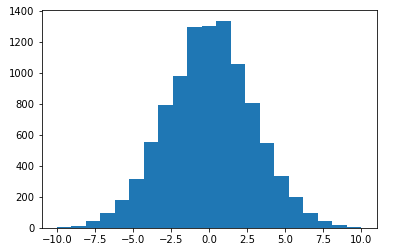
\includegraphics[width=\linewidth]{gauss.png}
  \caption{Profil d'une notation centrée autour de 0, distribution sur 10000 tirages}
  % \vspace{-15pt}
\end{figure}



\paragraph{Profil extrême}


\begin{figure}[ht]
  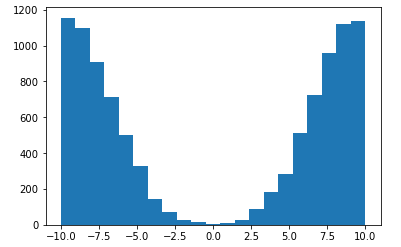
\includegraphics[width=\linewidth]{antigauss.png}
  \caption{Profil d'une notation polarisante, distribution sur 10000 tirages}
  % \vspace{-15pt}
\end{figure}

\paragraph{D'autres profils possibles}

trimodal

\paragraph{Résultats}

Pour les trois profils, les simulations donnent un indicateur \gls{bsn} suivant un loi gaussienne centrée, pour 10 et 100 ajouts de nouvelles comparaisons.
Concernant le \gls{EAM}, pour les trois profils, les simulations montrent que l'écart entre l'heuristique et l'algorithme Mehestan est important pour l'ajout de 10 nouvelles comparaisons. Toutefois, cet écart s'amenuise pour 100 nouvelles comparaisons.


\subsubsection{Evaluation sur données réelles}


\paragraph{Méthodologie}

Pour évaluer l'heuristique sur les données publiques de Tournesol, à volumétrie réelle, la démarche en quatre étapes est la suivante :

\begin{enumerate}
    \item Chargement de la base de données publiques
    \item Modifications préalable
    \item Tirage de l'échantillon
    \item Tirs sur l'application
\end{enumerate}
L'évaluation de l'heuristique a été réalisé en environnement de developpement en local pour éviter les effets de réseau avec une volumétrie réelle, soit 3x xxx comparaisons.
Dans un premier temps, il est nécessaire de réinitialiser la base de données de développement, puis de charger les données publiques par Django à l'aide de la fonctionnalité dédiée.

Dans un second temps, afin de faciliter l'automatisation, les noms d'utilisateurs des contributeurs ont été renommés de user1 à usern et leur mot de passe réinitialisé à "tournesolpassword". De manière similaire, les entités sont renommés de yt:00000000001 à yt:000000nnnnn. Les contributeurs ayant plus de 1000 comparaisons ont été promus "supertrusted", attribut non public servant de base de sondage pour la mise en place du réétalonnage.

Ensuite, parmi tous les couples (utilisateur, entité, notation), un échantillon de xx xxx n-uplets a été tiré en suivant une loi uniforme.

Enfin, à partir de l'échantillon tiré, le logiciel xh effectue chaque comparaison, de manière automatisée, à la place du conttributeur.


\paragraph{Résultats}

\pagebreak